\documentclass[twoside,a4paper,11pt]{article}
\setlength{\oddsidemargin}{0.25 in}
\setlength{\evensidemargin}{-0.25 in}
\setlength{\topmargin}{-0.6 in}
\setlength{\textwidth}{6.5 in}
\setlength{\textheight}{8.5 in}
\setlength{\headsep}{0.75 in}
\setlength{\parindent}{0 in}
\setlength{\parskip}{0.1 in}

%
% ADD PACKAGES here:
%
\usepackage[utf8]{inputenc} %for UTF8-extended encoding
\usepackage{amsmath,amsfonts,amssymb,graphicx,mathtools,flexisym}
\usepackage{caption} %for figures and labels captions
\usepackage{pbox} %to break the cell text in tables
\usepackage[skins,theorems]{tcolorbox} %to create color boxes for examples and recap

\usepackage[colorinlistoftodos,prependcaption,textsize=tiny]{todonotes}
\usepackage{tikz}
\usetikzlibrary{patterns}

\captionsetup{labelsep=space}
%
% The following commands set up the lecnum (lecture number)
% counter and make various numbering schemes work relative
% to the lecture number.
%
\newcounter{lecnum}
\renewcommand{\thepage}{\thelecnum-\arabic{page}}
\renewcommand{\thesection}{\thelecnum.\arabic{section}}
\renewcommand{\theequation}{\thelecnum.\arabic{equation}}
\renewcommand{\thefigure}{\thelecnum.\arabic{figure}}
\renewcommand{\thetable}{\thelecnum.\arabic{table}}

%
% The following macro is used to generate the header.
%
\newcommand{\lecture}[5]{
   \pagestyle{myheadings}
   \thispagestyle{plain}
   \newpage
   \setcounter{lecnum}{#1}
   \setcounter{page}{1}
   \noindent
   \begin{center}
   {\bf COVENTRY UNIVERSITY}
   \framebox{
      \vbox{\vspace{2mm}
    \hbox to 6.28in { {\bf 208MED: Mechanics
	\hfill Spring 2019} }
       \vspace{4mm}
       \hbox to 6.28in { {\Large \hfill Lecture #1: #2  \hfill} }
       \vspace{2mm}
       \hbox to 6.28in { {\textsl{#3} \hfill \texttt{#4}} }
      \vspace{2mm}}
   }
   \end{center}
   \markboth{Lecture #1: #2}{Lecture #1: #2}

%   {\bf Note}: {\it LaTeX template courtesy of UC Berkeley EECS dept.}

   {\bf Disclaimer}: {\it These notes have not been subjected to the
   usual scrutiny reserved for formal publications.  They may be distributed
   outside this class only with the permission of the instructor.}
   \vspace*{4mm}
}

% **** IF YOU WANT TO DEFINE ADDITIONAL MACROS FOR YOURSELF, PUT THEM HERE:


\begin{document}
%FILL IN THE RIGHT INFO.
%\lecture{**LECTURE-NUMBER**}{**DATE**}{**LECTURER**}{**SCRIBE**}
\lecture{01}{Mechanics revision}{Dr. Arnaldo Delli-Carri}{ac4213@coventry.ac.uk}
%\footnotetext{These notes are partially based on those of R. C. Hibbeler}

\tableofcontents

% **** YOUR NOTES GO HERE:

\section{Equilibrium}
Since statics plays an important role in both the development and application of mechanics of materials, it is very important to have a good grasp of its fundamentals. For this reason we will now review some of the main principles of statics that will be used throughout the text.
\subsection{Active forces}
A body can be subjected to both surface loads and body forces. Surface loads that act on a small area of contact are reported by concentrated forces, while distributed loadings act over a larger surface area of the body. When the loading is coplanar (i.e. 2D) as in Figure \ref{fig:LoadedBeam}, then a resultant force $F_R$ of a distributed loading is equal to the area under the distributed loading diagram, and this resultant acts through the geometric center or \emph{centroid} of that area.

\begin{figure}[!h]
\centering
\begin{tikzpicture}
%constraints
\draw[thick,fill=black] (0,-0.2) -- ++(-60:0.2) -- ++(180:0.2) -- cycle;
\draw[fill=black] (4.5,-0.2) ++(-90:0.15) circle (0.15);
\draw[fill=black] (0,-0.2) node[left]{$A$} -- ++(-60:0.3) -- ++(180:0.3) -- cycle;
%loads
\foreach \x in {0,0.2,...,2} {
	\draw[latex-] (\x,0) -- ++(0,0.5); }
\draw (0,0.5) -- ++(2,0)  node[pos=0.5,above] {\small $200$N/m};
\draw[thick,latex-] (3.5,0) -- ++(0,1) node[above]{$200$N};
%beam
\draw[thick,fill=black!40] (0,0) rectangle (4.5,-0.2) node[right]{$B$};
%dimensions
\draw[help lines,latex-latex] (0,-0.6) -- ++(2,0) node[fill=white,midway]{\footnotesize 2m};
\draw[help lines,latex-latex] (2,-0.6) -- ++(1.5,0) node[fill=white,midway]{\footnotesize 1.5m};
\draw[help lines,latex-latex] (3.5,-0.6) -- ++(1,0) node[fill=white,midway]{\footnotesize 1m};
%RIGHT FIGURE
\begin{scope}[xshift=7cm]
%constraints
%loads
\foreach \x in {0,0.2,...,0.8,1.2,1.4,...,2} {
	\draw[black!30,latex-] (\x,0) -- ++(0,0.5);
}
\draw[black!30] (0,0.5) -- ++(2,0)  node[pos=0,above,yshift=-0.1cm] {\small $200$N/m};
\draw[thick,latex-] (1,0) -- ++(0,0.9) node[text width=3cm, text centered,above]{$400$N \\ $\left( 200 \text{N/m} \times 2 \text{m} \right)$};
\draw[thick,latex-] (3.5,0) -- ++(0,1) node[above]{$200$N};
\draw[red,thick,latex-] (0,-0.3) -- ++(0,-1) node[right] {$A_y$};
\draw[red,thick,-latex] (-0.5,-1) -- ++(1,0) node[right] {$A_x$};
\draw[red,thick,latex-] (4.5,-0.3) -- ++(0,-1) node[right] {$B_y$};
%beam
\draw[thick,fill=black!40] (0,0) rectangle (4.5,-0.2) node[right]{$B$};
%dimensions
\draw[help lines,latex-latex] (0,-0.6) -- ++(1,0) node[fill=white,midway]{\footnotesize 1m};
\draw[help lines,latex-latex] (1,-0.6) -- ++(1,0) node[fill=white,midway]{\footnotesize 1m};
\draw[help lines,latex-latex] (2,-0.6) -- ++(1.5,0) node[fill=white,midway]{\footnotesize 1.5m};
\draw[help lines,latex-latex] (3.5,-0.6) -- ++(1,0) node[fill=white,midway]{\footnotesize 1m};
\end{scope}
\end{tikzpicture}
\caption{A loaded beam (left) and its Free Body Diagram (right)}
\label{fig:LoadedBeam}
\end{figure}

For other type of distributed loadings (Table \ref{tab:DistLoads}), the resultant can be found by integrating the distribution function over the length of application and the centroid using the equilibrium of moments. 

\begin{center}
\begin{tabular}[htb]{|c|c|c|c|}
	\hline
	\textbf{Name} & \textbf{Loading} & \textbf{Resultant} & \textbf{Centroid} \\
	\hline
Rectangular &\begin{tikzpicture}[baseline]
\foreach \x in {0,0.25,...,3} {
	\draw[cyan,latex-] (\x,0) -- ++(0,0.5);
} \draw[cyan] (0,0.5) node[left]{$q$} -- +(3,0);
\draw (0,0) -- (3,0);
\draw[thick,latex-] (1.5,0) -- +(0,1) node[right]{$F$};
\draw[help lines,latex-latex] (0,-0.3) -- +(1.5,0) node[midway,fill=white]{$x'$}; 
\draw[help lines,latex-latex] (0,-0.6) -- +(3,0) node[fill=white,pos=0.7]{$L$}; 
 \end{tikzpicture}	 & $F=qL$ & $x'=\dfrac{L}{2}$ \\
 \hline
Triangular &	\begin{tikzpicture}[baseline]
	\foreach \x in {0.4,0.6,0.8,1,1.2,1.4,1.6,1.8,2.2,2.4,2.6,2.8,3} {
		\draw[cyan,latex-] (\x,0) -- ++(0,\x*0.5);
	} \draw[cyan](0.2,0) -- +(0,0.2*0.5); 
\draw[cyan] (0,0) -- +(3,0.5*3) node[below right]{$q$};
\draw (0,0) -- (3,0);
	\draw[thick,latex-] (2,0) -- +(0,1.5) node[left]{$F$};
	\draw[help lines,latex-latex] (0,-0.3) -- +(2,0) node[midway,fill=white]{$x'$}; 
	\draw[help lines,latex-latex] (0,-0.6) -- +(3,0) node[fill=white,pos=0.8]{$L$}; 
	\end{tikzpicture} & $F=\dfrac{qL}{2}$ & $x'=\dfrac{2}{3}L$ \\
	\hline
Generic & \begin{tikzpicture}[baseline]
    \pgfmathsetseed{2}
    \draw[cyan]plot[smooth, samples=5,domain={0:3}] (\x,rnd+0.05) node[at start,above=0.3cm]{$q(x)$}; 
    \draw[cyan,latex-] (0,0) -- (0,0.3);
    \draw[cyan,latex-] (3,0) -- (3,0.8);
	\draw (0,0) -- (3,0);
	\draw[thick,latex-] (2.3,0) -- +(0,1.5) node[left]{$F$};
	\draw[help lines,latex-latex] (0,-0.3) -- +(2.3,0) node[midway,fill=white]{$x'$}; 
	\draw[help lines,latex-latex] (0,-0.6) -- +(3,0) node[fill=white,pos=0.5]{$L$}; 
	\end{tikzpicture} & $F=\displaystyle\int_L q(x)\,\mathrm{d}x$ & $x'=\displaystyle\frac{\displaystyle\int_L xq(x)\,\mathrm{d}x}{\displaystyle\int_L q(x)\,\mathrm{d}x}$ \\
	\hline
\end{tabular}
\captionof{table}{Distributed loadings}
\label{tab:DistLoads}
\end{center}

A body force is developed when a body exerts a force on another body without direct physical contact between them. Examples include the effects caused by the Earth's gravitation or its electromagnetic field. Although these forces affect all particles composing the body, they are normally represented by a single concentrated force acting on the body. In the case of gravitation, this force is called the weight $W$ of the body and acts through the body's centre of gravity.

\subsection{Constraints and reactive forces}
For bodies subjected to coplanar force systems, the supports most commonly encountered are shown in Table \ref{tab:Constraints}. As a general rule, if the support prevents translation in a given direction, then a force must be developed on the member in that direction. Likewise, if rotation is prevented, a couple moment must be exerted on the member. For example, the roller support only prevents translation perpendicular or normal to the surface. Hence, the roller exerts a normal force F on the member at its point of contact. Since the member can freely rotate about the roller, a couple moment cannot be developed on the member.

\begin{center}
	\begin{tabular}[htb]{|c|c||c|c|}
		\hline
		\textbf{Name} & \textbf{Constraint} & \textbf{Name} & \textbf{Constraint} \\
		\hline
		Roller &\begin{tikzpicture}[baseline,rotate=-45]
	\begin{scope}
		\clip (0,0) rectangle (2,1);
		\draw[thick] (0,0) -- (45:3);
	\end{scope}
		\draw[fill=white] (0,0) ++(-60:0.3) ++(180:0.1) circle (2pt);
		\draw[fill=white] (0,0) ++(-60:0.3) ++(180:0.2) circle (2pt);
		\draw[fill=black] (0,0) -- ++(-60:0.3) -- ++(180:0.3) -- cycle;
     	\draw[fill=white] (0,0) circle (2pt);
     	\draw[ultra thin] (-0.5,-0.35) -- ++(1,0);
		\draw[red,latex-] (0,-0.35) -- +(0,-0.7) node[right]{$R$};
		\draw[thin,green!70!black,<->] (-0.4,-0.2) -- +(0.8,0);
		\draw[thin,green!70!black,<->] (10:0.5) arc (10:80:0.5);
		\end{tikzpicture}	 
		& Sliding collar & \begin{tikzpicture}[baseline]
		\begin{scope}
		\clip (0,0) rectangle (2,1);
		\draw[thick](0,0) -- (3,1.3);
		\end{scope}
		\draw[fill=white] (-0.1,-0.15) circle (2pt);
		\draw[fill=white] (0.1,-0.15) circle (2pt);
		\draw[fill=black] (-0.2,0) rectangle +(0.4,-0.1);
     	\draw[ultra thin] (-0.5,-0.22) -- ++(1,0);
		\draw[red,latex-] (0,-0.3) -- +(0,-0.7) node[right]{$R$};
		\draw[green!70!black,<->] (-0.4,-0.06) -- +(0.8,0);
		\draw[red,-latex] (-130:0.5) arc (-130:-40:0.5) node[at end,right,yshift=-0.1cm] {$M$};
		\end{tikzpicture}\\
		\hline
		Pin &	\begin{tikzpicture}[baseline]
		\begin{scope}
		\clip (0,0) rectangle (2,1);
		\draw[thick] (0,0) -- (20:3);
		\end{scope}
		\draw[fill=black] (0,0) -- ++(-60:0.3) -- ++(180:0.3) -- cycle;
		\draw[fill=white] (0,0) circle (2pt);
		\draw[red,latex-] (0,-0.3) -- +(0,-0.7) node[right]{$R_y$};
     	\draw[red,-latex] (-0.5,-0.5) -- +(1,0) node[right]{$R_x$};
		\draw[thin,green!70!black,<->] (-20:0.5) arc (-20:60:0.5);
		\end{tikzpicture} & Pantograph &  \begin{tikzpicture}[baseline]
		\begin{scope}
		\clip (0,0) rectangle (2,1);
		\draw[thick] (0,0) -- (20:3);
		\end{scope}
		\begin{scope}[yshift=-0.37cm]
		\draw[fill=white] (-0.1,0) circle (1.5pt);
		\draw[fill=white] (0.1,0) circle (1.5pt);
		\draw[thick] (-0.1,0) -- ++(40:0.2) -- +(140:0.2);
		\draw[thick] (0.1,0) -- ++(40:0.2) -- +(140:0.2);
		\draw[fill=white] (-0.1,0) circle (1.5pt); \draw[fill=white] (0.1,0) circle (1.5pt);
		\draw[fill=white] (-0.1,0) ++(40:0.2) circle (1.5pt); \draw[fill=white] (0.1,0) ++(40:0.2) circle (1.5pt);
		\draw[fill=white] (-0.1,0) ++(40:0.2) +(140:0.2) circle (1.5pt); \draw[fill=white] (0.1,0) ++(40:0.2) +(140:0.2) circle (1.5pt);
		\draw[ultra thin] (-0.5,-0.06) -- ++(1,0);
		\draw[fill=black] (-0.3,0) ++(40:0.2) ++(140:0.2) +(0,0.05) rectangle +(0.6,0.1);
		\end{scope}
		\draw[green!70!black,<->] (0.6,0.37) -- +(0.8,0);
		\draw[green!70!black,<->] (1,0) -- +(0,0.8);
		\draw[red,-latex] (-130:0.8) arc (-130:-40:0.8) node[at end,right,yshift=-0.1cm] {$M$};
		\end{tikzpicture}  \\
		\hline
		Fixed & \begin{tikzpicture}[baseline]
		\begin{scope}
		\clip (0,0) rectangle (2,1);
		\draw[thick] (0,0) -- (20:3);
		\end{scope}
		\draw[fill=black] (-0.1,-0.3) rectangle ++(0.1,0.6);
		\draw[red,latex-] (-0.15,0) -- +(-0.7,0) node[above]{$R_x$};
		\draw[red,latex-] (0,-0.3) -- +(0,-0.7) node[right]{$R_y$};
		\draw[red,-latex] (100:0.5) arc (100:260:0.5) node[midway,below,xshift=-0.1cm,yshift=-0.2cm] {$M$};
		\end{tikzpicture} & 
		Free &  \begin{tikzpicture}[baseline]
		\begin{scope}
		\clip (0,-1) rectangle (2,1);
		\draw[thick] (0,0) -- (20:3);
		\end{scope}
		\draw[green!70!black,<->] (-0.4,0) -- +(0.8,0);
		\draw[green!70!black,<->] (0,-0.4) -- +(0,0.8);
		\draw[thin,green!70!black,<->] (-20:0.7) arc (-20:60:0.7);	
		\end{tikzpicture} \\
		\hline
	\end{tabular}
	\captionof{table}{2D-constraints}
	\label{tab:Constraints}
\end{center}

\subsection{Equilibrium equations}
Equilibrium of a body requires both a balance of forces, to prevent the body from translating or having accelerated motion along a straight or curved path, and a
balance of moments, to prevent the body from rotating. These conditions are expressed mathematically as the equations of equilibrium:

\begin{equation}
\tcbhighmath[arc=1pt,colframe=green!50!black,colback=green!10!white]{
\begin{cases}
\sum{\mathbf{F}}=\mathbf{0} \\
\sum{\mathbf{M}_P}=\mathbf{0}
\end{cases}
}
\end{equation}

Here, $\sum{\mathbf{F}}$ represents the sum of all the forces acting on the body, and
$\sum{\mathbf{M}_P}$ is the sum of the moments of all the forces about \emph{any} point $P$ either on or off the body. If an $xyz$ coordinate system is established with the origin at point $P$, the force and moment vectors can be resolved into components along each coordinate axis, and the above two equations can be written in
scalar form as six equations, namely,
\begin{equation}
\begin{cases}
\sum{F_x}=0 \qquad \mbox{translation along the x-axis}\\ 
\sum{F_y}=0 \qquad \mbox{translation along the y-axis}\\ 
\sum{F_z}=0 \qquad \mbox{translation along the z-axis}\\ 
\sum{M_x}=0 \qquad \mbox{rotation around the x-axis}\\ 
\sum{M_y}=0 \qquad \mbox{rotation around the y-axis}\\ 
\sum{M_z}=0 \qquad \mbox{rotation around the z-axis}
\end{cases}
\end{equation}

Often in engineering practice the loading on a body can be represented as a system of coplanar forces in the $xy$-plane. In this case equilibrium of the body can be specified with only three scalar equilibrium equations, that is,
\begin{equation}
\begin{cases}
\sum{F_x}=0 \qquad \mbox{translation along the x-axis}\\ 
\sum{F_y}=0 \qquad \mbox{translation along the y-axis}\\ 
\sum{M_P}=0 \;\;\quad \mbox{rotation around the z-axis passing through $P$}\\ 
\end{cases}
\end{equation}

Successful application of the equations of equilibrium must include all the known and unknown forces that act on the body, and the best way to account for these loadings is to draw the structure's free-body diagram before applying the equations of equilibrium. For example, the free-body diagram of a beam is shown in Fig. \ref{fig:LoadedBeam}. Here each force is identified by its magnitude and direction, and the beam dimensions are included in order to sum the moments of the forces. 

\section{Internal forces} \label{fig:SecInternalForces}
In mechanics of materials, statics is primarily used to determine the resultant loadings that act within a body. This is done using the \emph{method of sections}. 

Consider the body shown in Fig. \ref{fig:InternalForces}, which is held in equilibrium by four external forces. In order to obtain the internal loadings acting on a specific region within the body, it is necessary to pass an imaginary section (i.e. cut) through the region where the internal loadings are to be determined. The two parts of the body are then separated, and a free-body diagram of one of the parts is drawn. When this is done, there will be a distribution of internal forces acting on the exposed area of the section (Fig. \ref{fig:InternalForces} (center). These forces actually represent the effects of the material of the top section of the body acting on the bottom section. Although the exact distribution of this internal loading may be unknown, its resultants $R$ and $R_M$ are determined by applying the equations of equilibrium to that segment. These internal resultants acts at the centroid of the sectioned area.

\begin{figure}[!h]
	\centering
	\begin{tikzpicture}
%FIRST FIGURE
	%beam
	\fill[inner color=white, outer color=blue!50, opacity=0.8] plot [smooth cycle] coordinates {(0,0) (0,0.5) (0,1) (1.2,1) (2,1) (2,0.5) (2,0) 
	(2,-0.5) (2,-1) (0,-1)  (0,-0.5)};
\draw[fill=white,opacity=0.3] (-1,-0.2) -- ++(4,0) -- ++(135:0.6) -- ++(180:3) -- cycle;
    \draw[thick,fill=cyan!50,opacity=0.3] (1,0) ellipse (1 and 0.2);
	%loads
	\draw[thick,-latex] (0,1) -- ++(-0.8,0.4) node[above]{$F_1$};
	\draw[thick,-latex] (1.5,0.8) -- ++(70:0.8) node[above]{$F_2$};
	\draw[thick,-latex] (0.3,-0.6) -- ++(220:0.8) node[below]{$F_3$};
    \draw[thick,-latex] (1.5,-0.8) -- ++(-80:0.7) node[below]{$F_4$};
	\draw (4,0) node[text width=2cm, text centered] {imaginary \\ section};
%SECOND FIGURE	
\begin{scope}[xshift=6cm]
\begin{scope}
\clip(-1,0) rectangle (3,-3);
\fill[inner color=white, outer color=blue!50, opacity=0.8] plot [smooth cycle] coordinates {(0,0) (0,0.5) (0,1) (1.2,1) (2,1) (2,0.5) (2,0) 
	(2,-0.5) (2,-1) (0,-1)  (0,-0.5)};
\end{scope}
%beam
\draw[thick,fill=white,opacity=0.3] (-1,-0.2) -- ++(4,0) -- ++(135:0.6) -- ++(180:3) -- cycle;
\draw[fill=cyan!40,opacity=1] (1,0) ellipse (1 and 0.2);
%loads
	\draw[thick,-latex] (0.3,-0.6) -- ++(220:0.8) node[below]{$F_3$};
\draw[thick,-latex] (1.5,-0.8) -- ++(-80:0.7) node[below]{$F_4$};
%internal
	\draw[thick,-latex,blue] (1,0) -- ++(72:1.3) node[above]{$R$};
    \draw[thick,>=latex,->>,red] (1,0) -- ++(140:1.5) node[above]{$R_M$};
\end{scope}
%THIRD FIGURE	
\begin{scope}[xshift=11cm]
\begin{scope}
\clip(-1,0) rectangle (3,-3);
\fill[inner color=white, outer color=blue!50, opacity=0.8] plot [smooth cycle] coordinates {(0,0) (0,0.5) (0,1) (1.2,1) (2,1) (2,0.5) (2,0) 
	(2,-0.5) (2,-1) (0,-1)  (0,-0.5)};
\end{scope}
%beam
\draw[thick,fill=white,opacity=0.3] (-1,-0.2) -- ++(4,0) -- ++(135:0.6) -- ++(180:3) -- cycle;
\draw[fill=cyan!40,opacity=1] (1,0) ellipse (1 and 0.2);
%loads
\draw[thick,-latex] (0.3,-0.6) -- ++(220:0.8) node[below]{$F_3$};
\draw[thick,-latex] (1.5,-0.8) -- ++(-80:0.7) node[below]{$F_4$};
%internal
\draw[thick,-latex,blue] (1,0) -- ++(90:1.6) node[above]{$N$};
\draw[thick,>=latex,->>,red!50!yellow] (1,0) -- ++(90:1) node[right]{$T$};
\draw[thick,-latex,green!70!black] (1,0) -- +(135:0.6) -- +(-45:0.6) node[pos=0,left]{$V$};
\draw[thick,>=latex,->>,red] (1,0) -- +(40:0.6) -- +(220:0.6) node[pos=0,right]{$M$};
\end{scope}
	
	\end{tikzpicture}
	\vspace{-1.2cm}
	\caption{}
	\label{fig:InternalForces}
\end{figure}


For later application of the formulas for solid mechanics, we will consider the components of $R$ and $R_M$ acting both normal and parallel to the sectioned area (Fig. \ref{fig:InternalForces} right).

Four different types of resultant loadings can then be defined as follows: 
\begin{itemize}
	\item Normal force, $\mathbf{N}$. This force acts perpendicular to the section. It is developed whenever the external loads tend to push or pull on the two segments of the body.
	\item Shear force(s), $\mathbf{V}$. The shear force lies in the plane of the section and it is developed when the external loads tend to cause the two segments of the body to slide over one another (i.e. like a deck of cards). There is just a single shear force acting in the plane of the section, but this can be furtherly split into two perpendicular components for ease of calculation.
	\item Bending moment(s), $\mathbf{M}$. The bending moment is caused by the external loads that tend to bend the body about an axis lying within the plane of the area. Notice that graphical representation of a moment or torque is shown in three dimensions as a vector (double arrow) with an associated curl around it. By the right-hand rule, the thumb gives the arrowhead sense of this vector
	and the fingers or curl indicate the tendency for rotation (twisting or bending). There is just a single bending moment acting around an axis in the plane of the section, but this can be furtherly split into two perpendicular components for ease of calculation.
	\item Torsional moment or twisting torque, $\mathbf{T}$. This effect is developed when the external loads tend to twist a segment of the body with respect to the other about an axis perpendicular to the area. 
\end{itemize}

If the body is subjected to a 2D system of forces, Fig. 13a, then only normal-force, shear-force, and bending moment components will exist at the section, Fig. 13b. If we use the $xyz$ coordinate axes, as shown on the left segment, then N can be obtained by applying $\sum{F_x}=0$, and V can be obtained from $\sum{F_y}=0$. Finally, the bending moment $M$ can be determined by summing moments about point O (the $z$ axis), $\sum{M_O}=0$, in order to eliminate the moments caused by the normal force $N$ and shear force $V$.

\section{Stresses and strains}
It was stated in Section \ref{fig:SecInternalForces} that the force and moment acting at the centroid of the sectioned area of the body (Fig. \ref{fig:InternalForces}) represents the resultant effects of the distribution of stresses that act over the sectioned area. Obtaining this stress distribution is of primary importance in mechanics of materials.

To solve this problem it is first necessary to establish the concept of stress. We begin by considering the sectioned area to be subdivided into small areas. As we reduce to a smaller and smaller size, we will make two assumptions regarding the properties of the material: we will consider the material to be continuous and cohesive, meaning that all portions of it are connected together, without having breaks, cracks, or separations. 

\begin{figure}[htb]
\centering

\begin{tikzpicture}[thick, scale=2]
\draw[fill=white] (0,0) rectangle (2,1);
\draw[fill=black!30] (2,0) -- ++(45:1.8) -- ++(0,1) -- ++(180+45:1.8) -- cycle;
\draw[fill=black!20] (0,1) -- ++(45:1.8) -- ++(2,0) -- ++(180+45:1.8) -- cycle;
\draw[green!70!black,-latex] (1,0.5) ++(0:0.6) -- ++(180:1.4) node[above]{$V_y$};
\draw[green!70!black,-latex] (1,0.5) ++(-90:0.4) -- ++(90:0.8) node[right]{$V_z$};
\draw[red!50!yellow,<-] (1,0.5) ++(180+45:0.6) ++(0.22,0.2) arc (20:-190:0.15) node[pos=0,right,yshift=-2pt] {$T$};
\draw[blue,-latex] (1,0.5) -- ++(180+45:0.9) node[below]{$N$};
\draw[red,<-] (1,0.5) ++(0.15,0.25) arc (-10:-190:0.15) node[pos=0,right,yshift=-2pt] {$M_z$};
\draw[red,->] (1,0.5) ++(-0.5,-0.15) arc (-100:-260:0.15) node[pos=1,above] {$M_y$};


\draw[fill=red] (1.6,0.15) rectangle +(0.1,0.1);
\draw[help lines] (1.65,0.2) circle (0.15cm);
\draw[help lines] (1.65,0.35) -- ++(33:3.4);
\draw[help lines] (1.65,0.05) -- ++(-4:3.35);

\begin{scope}[xshift=4.5cm,yshift=0.3cm]
\draw[thin,help lines] (0.7,0.8) circle (1.3cm);
\draw[fill=white] (0,0) rectangle (1,1);
\draw[fill=white] (1,0) -- ++(0.5,0.5) -- ++(0,1) -- +(-0.5,-0.5) -- cycle;
\draw[fill=white] (0,1) -- ++(0.5,0.5) -- ++(1,0) -- +(-0.5,-0.5) -- cycle;
%axes
\draw[-latex,thin] (0,0) -- +(-0.15,-0.15) node[right]{$x$};
\draw[-latex,thin] (1.5,0.5) -- +(0.3,0) node[below]{$y$};
\draw[-latex,thin] (0.5,1.5) -- +(0,0.3) node[right]{$z$};
%stresses front face
\draw[-latex][color=green!50!black] (0.1,0.5) -- +(0.8,0) node[below left] {$\tau_{xy}$};
\draw[-latex][color=green!50!black] (0.5,0.1) -- +(0,0.8) node[below right] {$\tau_{xz}$};
\draw[-latex][color=blue] (0.5,0.5) -- +(-0.25,-0.25) node[below] {$\sigma_{xx}$};
%stresses lateral face
\draw[latex-][color=green!50!black] (1.05,0.55) node[below=-3pt,xshift=0.17cm] {$\tau_{yx}$} -- +(0.4,0.4) ;
\draw[-latex][color=green!50!black] (1.25,0.35) -- +(0,0.8) node[right=-3pt] {$\tau_{yz}$};
\draw[-latex][color=blue] (1.25,0.75) -- +(0.5,0) node[above] {$\sigma_{yy}$};
%stresses upper face
\draw[-latex][color=green!50!black] (0.35,1.25) -- +(0.8,0) node[below left=-1pt,xshift=-1pt] {$\tau_{zy}$};
\draw[latex-][color=green!50!black] (0.55,1.05) node[above left=-1pt] {$\tau_{zx}$} -- +(0.4,0.4);
\draw[-latex][color=blue] (0.75,1.25) --+(0,0.5) node[right] {$\sigma_{zz}$};
\end{scope}
\end{tikzpicture}
\caption{stress element (infinitesimal)}
\label{fig:StressCube}
\end{figure}

A typical finite yet very small force $\Delta F$, acting on $\Delta A$, is shown in Fig. This force, like all the others, will have a unique direction, but can always be split into its three components, namely $\Delta F_x$, $\Delta F_y$, and $\Delta F_z$. As $\Delta A$ approaches zero, so do $\Delta F$ and its components; however, the quotient of the force and area will approach a finite limit. 

This quotient is called \emph{stress}, and it describes the intensity of the internal force acting on a specific plane (area) passing through a point.

The intensity of the force acting normal to $\Delta A$ is
referred to as the {\bf\emph{normal} stress}, $\sigma$ (sigma). Since $\Delta F_z$ is normal to the area then

\begin{equation}
\sigma_x=\lim_{\Delta A \rightarrow 0} \frac{\Delta F_x}{\Delta A}
\end{equation}

If the normal force or stress "pulls" on $\Delta A$ as shown in Fig. 19a, it is \emph{tensile} stress, whereas if it "pushes” on $\Delta A$ it is \emph{compressive} stress.

The intensity of force acting tangent to $\Delta A$ is called the {\bf\emph{shear} stress}, $\tau$ (tau). Here we have two shear stress components due to two component of the force $\Delta F$ acting parallel to the section plane.

\begin{align}
\tau_{xy} &= \lim_{\Delta A \rightarrow 0} \frac{\Delta F_y}{\Delta A} \\
\tau_{xz} &= \lim_{\Delta A \rightarrow 0} \frac{\Delta F_z}{\Delta A} 
\end{align}

The first subscript $z$ specifies the orientation of the axis normal to the area $\Delta A$, while the second subscript $x$ or $y$ indicates the axes along which each shear stress acts, parallel to that area.

Finally, If the body is further sectioned by planes parallel to the $xz$-plane and the $yz$-plane, we can then "carve out" a cubic volume element of material that represents the {\bf \emph{stress state}} acting around a chosen point in the body. This state of stress is then characterized by three components acting on each face of the element, Fig.

\begin{figure}[hbt]
\centering
\begin{tikzpicture}
\fill[black!10] (0,0) -- ++(2,0) -- ++(1,1) -- ++(-2,0) -- cycle node[black,above right=0.5cm,xshift=0.1cm]{$\Delta A$};
\draw[thick,-latex] (1.5,0.5) -- ++(40:2) node[right] {$\Delta F$};
\draw[help lines,dashed] (1.5,0.5) ++(40:2) -- ++(0,-2) -- ++(0.6,0.6) ++(-2.1,0) ++(-0.6,-0.6) -- ++(2.1,0);
\draw[green!50!black,thick,-latex] (1.5,0.5) -- ++(-0.7,-0.7)  node[below left] {$\Delta F_y$};
\draw[green!50!black,thick,-latex] (1.5,0.5) -- ++(2.15,0)  node[right] {$\Delta F_z$};
\draw[help lines,dashed] (1.5,0.5) ++(40:2) ++(0,-2) -- (1.5,0.5);
\draw[help lines,dashed] (1.5,0.5) ++(40:2) -- (1.5,2.5);
\draw[blue,thick,-latex] (1.5,0.5) -- (1.5,2.5)  node[left] {$\Delta F_x$};
\end{tikzpicture}
\caption{}
\label{fig:SmallArea}
\end{figure}

\subsection{Average normal and shear stress}
Many engineering materials may be approximated as being both homogeneous and isotropic. Steel, for example, contains thousands of randomly oriented crystals in each cubic millimetre of its volume, and since most objects made of this material have a physical size that is very much larger than a single crystal, the assumption regarding the material's composition is quite realistic. 

Note that anisotropic materials, such as wood, have different properties in different directions; and although this is the case, if the fibers of wood are oriented along the beam's axis (as for instance in a typical wood board), then the bar will also deform uniformly when subjected to an axial load.

As a result, each small area $\Delta A$ on the cross section is subjected to a force $\Delta N = \sigma\cdot\Delta A$ and the sum of these forces acting over the entire cross-sectional area must be equivalent to the internal resultant force $N$ at the section. If we let $\Delta A \rightarrow dA$ and therefore $\Delta N \rightarrow dN$, then,
recognizing $\sigma$ is constant, we have 

\begin{align}
\int_A dN &=\int_A \sigma\cdot dA \\
N &=\sigma\cdot A
\end{align}

and finally 

\begin{equation}
\tcbhighmath[arc=1pt,colframe=green!50!black,colback=green!10!white]{\sigma = \frac{N}{A}}
\end{equation}

Where
\begin{description}
\item[$\sigma$] average normal stress at any point on the cross-sectional area

\item[$N$] internal resultant normal force, which acts through the centroid of the cross-sectional area. $N$ is determined using the method of sections and the equations of equilibrium

\item[$A$] cross-sectional area of the bar where $\sigma$ is determined
\end{description}

Under the condition of single axial loading, the material is said to be subjected to \emph{uniaxial} stress, and this analysis applies to members subjected to either tension or compression.

%SHEAR STRESS
Shear stress has been defined in Section x.x as the stress component that acts \emph{in the plane} of the sectioned area. Similarly to the normal stress, the \emph{average} shear stress distributed over each sectioned area that develops this shear force is defined by 
\begin{equation}
\tau_{avg} =\frac{V}{A}
\label{eq:TauAvg}
\end{equation}

Here
\begin{description}
\item[$\tau_{avg}$] average shear stress at the section, which is assumed to be the same at each point on the section
\item[$V$] internal resultant shear force on the section determined from the equations of equilibrium
\item[$A$] area of the section
\end{description}

Average shear stress is just an approximation, but it is useful to measure the stress condition of bolted, pinned and glued connections. The actual shear stress distribution is a more complex matter that will be discussed later. Finally, notice that $\tau_{avg}$ is in the same direction as $V$, since the shear stress must create associated forces, all of which contribute to the internal resultant force $V$.

The loading case discussed here is an example of simple or \emph{direct} shear, since the shear is caused by the direct action of the applied load. This type of shear often occurs in various types of simple connections that use bolts, pins, nails, welding material, etc. {\bf In all these cases, however, application of Eq. \ref{eq:TauAvg} is only approximate!}.

It is very important to notice that the developing of shear stress at an interface must be balanced by \emph{three} more shear components. In order to be in equilibrium, a 2D square infinitesimal element must

\begin{figure}
\centering

\begin{tikzpicture}[thick, scale=2]

\begin{scope}[xshift=0,yshift=0]
\draw[fill=white] (0,0) rectangle (1,1);
\draw[thin,-latex] (0.5,0.5) -- +(0,0.3) node[left]{$y$};
\draw[thin,-latex] (0.5,0.5) -- +(0.3,0) node[above]{$x$};
%stresses front face
\draw[-latex][color=green!50!black] (0.1,1.1) -- +(0.7,0) node[above] {$\tau_{yx}$};
\draw[->,red,dashed,thin] (0.1,0.2) -- +(0.8,0);
\draw[->,red,dashed,thin] (0.85,0.5) arc (0:-180:0.35);
\end{scope}

\begin{scope}[xshift=2cm,yshift=0]
\draw[fill=white] (0,0) rectangle (1,1);
\draw[thin,-latex] (0.5,0.5) -- +(0,0.3) node[left]{$y$};
\draw[thin,-latex] (0.5,0.5) -- +(0.3,0) node[above]{$x$};
%stresses front face
\draw[-latex,green!50!black] (0.1,1.1) -- +(0.7,0) node[above] {$\tau_{yx}$};
\draw[latex-,green!50!black] (0.1,-0.1) -- +(0.7,0) node[below] {$\tau_{yx}$};
\draw[->,red,dashed,thin] (0.85,0.5) arc (0:-180:0.35);
\end{scope}

\begin{scope}[xshift=4cm,yshift=0]
\draw[fill=white] (0,0) rectangle (1,1);
\draw[thin,-latex] (0.5,0.5) -- +(0,0.3) node[left]{$y$};
\draw[thin,-latex] (0.5,0.5) -- +(0.3,0) node[above]{$x$};
%stresses front face
\draw[-latex][color=green!50!black] (0.1,1.1) -- +(0.7,0) node[above] {$\tau_{yx}$};
\draw[latex-][color=green!50!black] (0.1,-0.1) -- +(0.7,0) node[below] {$\tau_{yx}$};
\draw[-latex][color=green!50!black] (1.1,0.1) -- +(0,0.7) node[above,xshift=0.1cm] {$\tau_{xy}$};
\draw[latex-][color=green!50!black] (-0.1,0.1) -- +(0,0.7) node[above,xshift=-0.1cm] {$\tau_{xy}$} ;
\end{scope}

\end{tikzpicture}

\caption{pure shear stress state: before equilibrium (left), after equilibrium of translations (center) and after equilibrium of rotations (right)}
\label{fig:ShearStress}
\end{figure}

All four shear stresses must have equal magnitude and be directed either toward or away from each other at opposite edges of the element, Fig. 1–20d. This is referred to as the {\bf \emph{complementary property of shear}}, and the element in this case is subjected to pure shear.

\subsection{Deformations and strains}
In order to describe the deformation of a body by changes in the lengths of line segments and changes in the angles between them, we will develop the concept of {\bf \emph{strain}}. Strain is actually measured experimentally, and once the strain is obtained, it can easily be linked to the stresses acting inside a body by using material properties and constitutive relationships.

\begin{figure}[hbt]
\centering
\begin{tikzpicture}
\draw[fill=black!20] (0,0) rectangle +(9,1);
\draw[thick,-latex] (-0.1,0.5) -- ++(-1,0) node[left]{$P$};
\draw[thick,-latex] (9.1,0.5) -- ++(1,0) node[right]{$P$};
\draw[fill=black!20] (0,-1.5) rectangle +(10,1);
\draw[thick,-latex] (-0.1,-1) -- ++(-1,0) node[left]{$P$};
\draw[thick,-latex] (10.1,-1) -- ++(1,0) node[right]{$P$};
\draw[help lines,latex-latex] (0,1.3) -- ++(9,0) node[midway,above]{$L_0$};
\draw[help lines,latex-latex] (9,1.3) -- ++(1,0) node[midway,above]{$\Delta L$};
\draw[help lines,latex-latex] (0,-2.1) -- ++(10,0) node[midway,above]{$L$};
\end{tikzpicture}
\caption{}
\label{fig:AxialBar}
\end{figure}
If an axial load $P$ is applied to the bar , it will change the bar’s length $L_0$ to a length $L$.
We will define the {\bf \emph{normal strain}} $\varepsilon$ (epsilon) of the bar as the change in its length $\Delta L = L-L_0$ divided by its original length, that is

\begin{equation}
\tcbhighmath[arc=1pt,colframe=green!50!black,colback=green!10!white]{\varepsilon = \frac{L-L_0}{L_0}=\frac{\Delta L}{L_0}}
\end{equation}

The normal strain $\varepsilon$ represents a change in length per unit length, and it is positive when the initial line elongates, and negative when it contracts.

Deformations not only cause line segments to elongate or contract, but they also cause them to change direction (distort). If we select two line segments that are originally perpendicular to one another, then the change in angle that occurs between them is referred to as {\bf\emph{shear strain}}. This angle is denoted by $\gamma$ (gamma) and is always measured in radians (rad), which are dimensionless.

\begin{figure}[hbt]
\centering

\begin{tikzpicture}[thick, scale=2]

\begin{scope}[xshift=2cm,yshift=0]
\draw[green!50!black] (0,0) rectangle (0.3,0.3) node[opacity=1,black,above]{$\frac{\pi}{2}$};
\draw (0,0) rectangle (1,1);
\end{scope}

\begin{scope}[xshift=4cm,yshift=0]
\draw[help lines,dashed] (0,0) rectangle (1,1);
\draw (0,0) -- (1,0) -- (1.5,1) -- (0.5,1) -- cycle;
\draw[blue] (0.3,0) arc (0:62:0.3) node[midway,right,yshift=0.1cm]{$\theta$};
\end{scope}

\begin{scope}[xshift=0cm,yshift=0]
\draw[help lines,dashed] (0,0) rectangle (1,1);
\draw (0,0) -- (1,0) -- (0.5,1) -- (-0.5,1) -- cycle;
\draw[red] (0.3,0) arc (0:118:0.3) node[midway,right,yshift=0.1cm]{$\theta$};
\end{scope}

\end{tikzpicture}

\caption{pure shear strain: negative shear strain (left), no shear (center) and positive shear strain (right)}
\label{fig:ShearStrain}
\end{figure}


For example, consider the two perpendicular line segments at a point in the block shown in Fig. If an applied loading causes the block to deform as shown in Fig. 2–3b, so that the angle between the line segments becomes $\theta$, then the shear strain at the point becomes

\begin{equation}
\tcbhighmath[arc=1pt,colframe=green!50!black,colback=green!10!white]{\gamma = \frac{\pi}{2} - \theta}
\end{equation}

Notice that if $theta$ is smaller than $\frac{\pi}{2}$, Fig. 2–3c, then the shear strain is positive, whereas if $theta$ is larger than $\frac{\pi}{2}$, then the shear strain is negative.

\subsection{Constitutive stress-strain relationships}
Stresses and strains are related through the so-called \emph{constitutive relationships} and \emph{material properties}.
The great majority of materials exhibit a stress-strain diagram that is linear until a \emph{proportional limit} has been hit. This region of proportionality is called \emph{elastic region} and this behaviour can be modelled using \emph{Hooke's Law}

\begin{equation}
\tcbhighmath[arc=1pt,colframe=green!50!black,colback=green!10!white]{\sigma = E \cdot \varepsilon}
\end{equation}

where $E$ represents the constant of proportionality, which is called the \emph{modulus of elasticity} or \emph{Young's modulus}, named after Thomas Young who published an account of it in 1807. Since strain is dimensionless, the units of the modulus of elasticity are the same of stress (i.e. $\left[\text{MPa}\right]$).

When a deformable body is subjected to a force, not only it does elongate but also contracts laterally. In the early 1800s, the french scientist Simeon Denis Poisson realised that \emph{within the elastic range} the \emph{ratio} of these strains is constant, since the deformations are proportional to the same applied force. This ratio is therefore referred to as \textbf{\emph{Poisson's ratio}} $\nu$ (nu) and has a value that is unique for any material that is both \emph{homogeneous} and \emph{isotropic}.

\begin{equation}
\tcbhighmath[arc=1pt,colframe=green!50!black,colback=green!10!white]{\nu=-\frac{\varepsilon_{lat}}{\varepsilon_{long}}}
\end{equation}

\begin{figure}[hbt]
\centering
\begin{tikzpicture}
\draw[help lines,dashed] (0,0) rectangle +(9,1.5);
\draw[fill=black!10] (-1,0.4) rectangle +(11,0.7);
\draw[thick,-latex] (-2,0.75) -- ++(-1,0) node[left]{$P$};
\draw[thick,-latex] (10.1,0.75) -- ++(1,0) node[right]{$P$};
\draw[help lines,latex-latex] (0,1.7) -- ++(9,0) node[midway,above]{$L_0$};
\draw[help lines,latex-latex] (-1,1.7) -- ++(1,0) node[midway,above]{$\frac{\Delta L}{2}$};
\draw[help lines,latex-latex] (9,1.7) -- ++(1,0) node[midway,above]{$\frac{\Delta L}{2}$};
\draw[help lines,latex-latex] (-1.5,1.1) -- +(0,0.4) node[midway,left]{$\frac{\Delta D}{2}$};
\draw[help lines,latex-latex] (-1.5,0.4) -- +(0,-0.4) node[midway,left]{$\frac{\Delta D}{2}$};
\draw[help lines,latex-latex] (-1.2,0) -- (-1.2,1.5) node[midway,left]{$D_0$};
\end{tikzpicture}
\caption{a positive longitudinal strain $\varepsilon_{long}=\frac{\Delta L}{L_0}$ causes a lateral strain $\varepsilon_{lat}=\frac{\Delta D}{D_0}$. Their quotient is the Poisson's ratio.}
\label{fig:AxialBar}
\end{figure}


The negative sign is included since in general \emph{longitudinal elongation} (positive strain) causes \emph{lateral contraction} (negative strain), and vice versa. Poisson's ratio is a dimensionless quantity and for most materials it has a value between 0.25 and 0.35.

For shear stresses and strains, the same linear relationship of normal stresses and strains exists, based on Hooke's law:

\begin{equation}
\tcbhighmath[arc=1pt,colframe=green!50!black,colback=green!10!white]{\tau = G \cdot \gamma}
\end{equation}

Here $G$ is called the \emph{shear modulus}. For isotropic materials, the three material constants discussed so far are not mutually independent, as they are related by the following expression:

\begin{equation}
\tcbhighmath[arc=1pt,colframe=green!50!black,colback=green!10!white]{G=\frac{E}{2\left(1+\nu\right)}}
\end{equation}

Therefore, for isotropic materials only two out of three elastic material properties need to be known in order to find all the possible relationships between stresses and strains.

\section{Axial loadings}
\subsection{De Saint-Venant's Principle}
Previously, we have developed the concept of stress as a means of measuring the force distribution within a body and strain as a means of measuring a body’s deformation. We have also shown that the mathematical relationship between stress and strain depends on the type of material from which the body is made. In particular, if the material behaves in a linear elastic manner, then Hooke’s law applies, and there is a proportional relationship between stress and strain.

Using this idea, consider the manner in which a rectangular bar will deform elastically when the bar is subjected to the force P applied along its centroidal axis, Fig. 4–1a. The once horizontal and vertical grid lines drawn on the bar become distorted, and localized deformation occurs at each end. Throughout the midsection of the bar, the lines remain
horizontal and vertical. 

\begin{figure}[hbt]
\centering
\begin{tikzpicture}
\draw[fill=black!10] (0,0) rectangle (1,5);
\draw[thick,-latex] (0.5,5.1) -- ++(0,0.5) node[right]{P};
\draw[thick,-latex] (0.5,-0.1) -- ++(0,-0.5) node[right]{P};
\draw[help lines,red] (-0.3,0.2) node[above]{$a$} -- (1.3,0.2)  node[above]{$a$};
\draw[help lines,blue] (-0.3,1) node[above]{$b$} -- (1.3,1)  node[above]{$b$};
\draw[help lines,green!50!black] (-0.3,2) node[above]{$c$} -- (1.3,2)  node[above]{$c$};

\begin{scope}[xshift=3cm]
\draw[fill=black!10] (0,0) rectangle (1,0.2);
\draw[thick,-latex] (0.5,-0.1) -- ++(0,-0.5) node[right]{P};
\draw[help lines,red] (-0.3,0.2) node[above]{$a$} -- (1.3,0.2)  node[above]{$a$};
\draw[red,domain=0:1,samples=100] plot ({\x},{0.1+exp(-(\x-0.5)*(\x-0.5)/(0.5*0.5))});
\foreach \x in {0,0.1,...,1.1}{
\draw[thin,red,-latex] (\x,0.2) -- (\x,{0.1+exp(-(\x-0.5)*(\x-0.5)/(0.5*0.5))});}
\end{scope}

\begin{scope}[xshift=6cm]
\draw[fill=black!10] (0,0) rectangle (1,1);
\draw[thick,-latex] (0.5,-0.1) -- ++(0,-0.5) node[right]{P};
\draw[help lines,blue] (-0.3,1) node[above]{$b$} -- (1.3,1)  node[above]{$b$};
\draw[blue,domain=0:1,samples=100] plot ({\x},{0.8+exp(-(\x-0.5)*(\x-0.5)/(1.1*1.1))});
\foreach \x in {0,0.1,...,1.1}{
\draw[thin,blue,-latex] (\x,1) -- (\x,{0.8+exp(-(\x-0.5)*(\x-0.5)/(1.1*1.1))});}
\end{scope}

\begin{scope}[xshift=9cm]
\draw[fill=black!10] (0,0) rectangle (1,2);
\draw[thick,-latex] (0.5,-0.1) -- ++(0,-0.5) node[right]{P};
\draw[help lines,green!50!black] (-0.3,2) node[above]{$c$} -- (1.3,2)  node[above]{$c$};
\draw[green!50!black,thin] (0,3) -- ++(1,0);
\foreach \x in {0,0.1,...,1.1}{
\draw[thin,green!50!black,-latex] (\x,2) -- (\x,3);}
\end{scope}

\end{tikzpicture}
\caption{De Saint-Venant principle: the stress distribution becomes more and more constant the further away the section is from the load application (border effect)}
\label{fig:SaintVenant}
\end{figure}


If the material remains elastic, then the strains caused by this deformation are directly related to the stress in the bar through Hooke’s law, $\sigma=E\varepsilon$. As a result, a profile of the variation of the stress distribution acting at sections a–a, b–b, and c–c, will look like that shown in Fig. 4–1b.

By comparison, the stress tends to reach a uniform value at section c–c, which is sufficiently removed from the end since the localized deformation caused by P vanishes. The minimum distance from the bar’s end where this occurs can be determined using a mathematical analysis based on the theory of elasticity. It has been found that this distance should at least be equal to the largest dimension of the loaded cross section. Hence, section c–c should be located at a distance at least equal to the width (not the thickness) of the bar.

In the same way, the stress distribution at the support in Fig. 4–1a will also even out and become uniform over the cross section located the same distance away from the support. The fact that the localized stress and deformation behave in this manner is referred to as {\bf\emph{Saint-Venant’s principle}}, since it was first noticed by the French scientist \emph{Barre de Saint-Venant} in 1855. Essentially it states that the stress and strain produced at points in a body sufficiently removed from the region of external load application will be the same as the stress and strain produced by any other applied external loading that has the same statically equivalent resultant and is applied to the body within the same region.

\subsection{Elastic deformation of an axially loaded member}
Using Hooke’s law and the definitions of stress and strain, we will now develop an equation that can be used to determine the elastic displacement of a member subjected to axial loads. To generalize the development, consider the bar shown in Fig. 4–2a, which has a cross-sectional area that gradually varies along its length L, and is made of a material that has a variable stiffness or modulus of elasticity. The bar is subjected to concentrated loads at its ends and a variable external load distributed along its length. This distributed load could, for example, represent the weight of the bar if it is in the vertical position, or friction forces acting on the bar’s surface. 

Here we wish to find the relative displacement $\Delta L$ of one end of the bar with respect to the other end as caused by the loading. We will neglect the localized deformations that occur at points of concentrated loading and where the cross section suddenly changes. From Saint-Venant’s principle, these effects occur within small regions of the bar’s length and will therefore have only a slight effect on the final result. For the most part, the bar will deform uniformly, so the normal stress will be uniformly distributed over the cross section.

\begin{figure}[hbt]
\centering
\begin{tikzpicture}

\draw[domain=0:8,samples=100] plot ({\x},{0.01*\x*\x}) -- (8,0);
\draw[domain=0:8,samples=100] (0,0) -- plot ({\x},{-1-0.01*\x*\x}) -- (8,0);
\draw[thick,-latex] (-0.1,-0.5) -- ++(-0.8,0) node[left]{$P_1$};
\draw[thick,-latex] (8.1,-0.5) -- ++(0.6,0) node[right]{$P_2$};
\draw(4.15,0.16) -- (4.15,-1.16);
\draw(4.95,0.25) -- (4.95,-1.25);
\fill[opacity=0.5,cyan] (4.15,0.16) -- (4.15,-1.16) -- (4.95,-1.25) -- (4.95,0.25);
\foreach \x in {0.2,0.6,...,7.8}{
\draw[thick,-latex] (\x,-0.5) -- +(0.32,0);}
\draw (6.5,-0.5) node[above=0.1cm]{$p(x)$};
%dimensions
\draw[latex-latex,help lines] (0,-2.5) -- +(8,0) node[midway, above]{$L_0$};
\draw[help lines](0,0.1) -- (0,0.6); \draw[-latex,help lines] (0,0.5) -- +(4.15,0) node[midway, above]{$x$};
\draw[latex-latex,help lines] (4.15,0.5) -- (4.95,0.5) node[midway, above]{$dx$};

\begin{scope}[xshift=12cm, yshift=-1.5cm]
\draw[help lines,dashed] (0,0) rectangle (1.5,2);
\draw[black,thick,fill=cyan!50] (0,0) rectangle (1,2);
\draw[thick,-latex] (-0.1,1) -- ++(-0.8,0) node[above]{$N(x)$};
\draw[thick,-latex] (1.6,1) -- ++(0.8,0) node[above]{$N(x)$};
\draw[latex-latex,help lines] (0,-0.5) -- (1,-0.5) node[midway, above]{$dx$};
\draw[latex-latex,help lines] (1,-0.5) -- (1.5,-0.5) node[midway, above]{$dL$};
\end{scope}

\end{tikzpicture}
\caption{}
\label{fig:AxialIntegral}
\end{figure}



Using the method of sections, an infinitesimal element of length $dx$ and cross-sectional area $A(x)$ is isolated from the bar at the arbitrary position $x$, where the modulus of elasticity is $E(x)$. The free-body diagram of this element is shown in Figure \ref{fig:AxialIntegral}. The resultant internal axial force will be a function of $x$ since the external distributed loading will cause it to vary along the length of the bar. This load $N(x)$ will deform the element into the shape indicated by the dashed outline, and therefore the displacement of one end of the element with respect to the other end becomes $dL$. The stress and strain in the element are therefore

\begin{equation}
\sigma =\frac{N(x)}{A(x)} \qquad\text{and}\qquad \varepsilon = \frac{dL}{dx}
\end{equation}


Provided the stress does not exceed the proportional limit, we can apply Hooke's law $\sigma=E\varepsilon$ and so

\begin{align}
\frac{N(x)}{A(x)} &= E(x)\cdot \frac{dL}{dx} \\
dL &= \frac{N(x)\cdot dx}{A(x)\cdot E(x)}
\end{align}

Integrating this expression over the entire original length $L_0$ of the bar, yields
\begin{equation}
\tcbhighmath[arc=1pt,colframe=green!50!black,colback=green!10!white]{\left(L-L_0\right)=\Delta L =\int_0^{L_0} \frac{N(x)}{E(x)A(x)}\,dx}
\label{eq:AxialEquation}
\end{equation}


Where
\begin{description}
\item[$\Delta L$] is the displacement of one end point on the bar relative to the other end point
\item[$L_0$]  is the original length of bar
\item[$N(x)$] is the internal axial force at the section, located a distance x from one end (found from the normal force diagram)
\item[$E(x)$] is the modulus of elasticity for the material varying over its length
\item[$A(x)$] is the cross-sectional area of the bar varying over its length
\end{description}

In many cases the bar will have a constant cross-sectional area $A$ and the material will be homogeneous so $E$ is constant. Furthermore, if a constant external force is applied at each end, then the internal force $N$ throughout the length of the bar is also constant. As a result, Eq. \eqref{eq:AxialEquation} when integrated becomes

\begin{equation}
\tcbhighmath[arc=1pt,colframe=green!50!black,colback=green!10!white]{\left(L-L_0\right)=\Delta L =\frac{NL_0}{EA}}
\end{equation}
If the bar is subjected to several different axial forces along its length, or the cross-sectional area or modulus of elasticity changes abruptly from one region of the bar to the next, then due to the integration rules the above equation can be applied once per each segment of the bar where these quantities remain constant. Often times, the quantity $\frac{EA}{L_0}$ is referred to as \emph{axial stiffness} of a bar.

\vspace{1cm}
\begin{tcolorbox}
	{\Large \bf Formulae sheet} \newline
	\begin{itemize}
		\item Equilibrium Equations
		\begin{equation*}		
			\begin{cases}
				\sum \mathbf{F} =\mathbf{0} \\
				\sum \mathbf{M}_P =\mathbf{0}
			\end{cases}
		\end{equation*}
		\item Normal stresses and strains
		\begin{equation*}		
			\sigma=\frac{N}{A}
		\end{equation*}
		\begin{equation*}		
			\varepsilon=\frac{L-L_0}{L_0}=\frac{\Delta L}{L_0}
		\end{equation*}
		\item Average shear stress and shear strain
		\begin{equation*}		
			\tau_{avg}=\frac{V}{A}
		\end{equation*}
		\begin{equation*}		
			\gamma=\frac{\pi}{2}-\theta
		\end{equation*}
		\item Constitutive relationships
		\begin{equation*}		
			\sigma=E\cdot\varepsilon \qquad \qquad \tau=G\cdot\gamma
		\end{equation*}
		\begin{equation*}		
			\nu=-\frac{\varepsilon_{lat}}{\varepsilon_{long}} \qquad \qquad G=\frac{E}{2(1+\nu)}
		\end{equation*}
		\item Axial loading
		\begin{equation*}
			\left(L-L_0\right)=\Delta L =\int_0^{L_0} \frac{N(x)}{E(x)A(x)}\,dx
		\end{equation*}
		\\
		if normal force, Young's modulus and cross-sectional area are constant, then
		\begin{equation*}
			\left(L-L_0\right)=\Delta L =\frac{NL_0}{EA}
		\end{equation*}
	\end{itemize}
\end{tcolorbox}

\end{document}